\begin{frame}{Tensor Network cut details}
\vskip-1.5cm

\begin{columns}[T]
  \begin{column}[T]{.5\textwidth}
  \only<1>{
  		\begin{figure}
			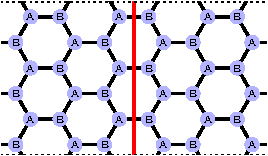
\includegraphics[width=\textwidth]{diagrams/Hex_PEPS.pdf}
			\caption{Generic honeycomb lattice PEPS on zig-zag cylinder with L=3}
		\end{figure}
		}
			\only<2>{
	  		\begin{figure}
			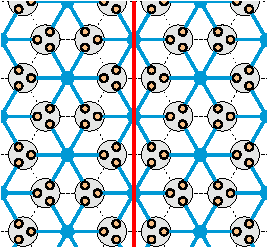
\includegraphics[width=\textwidth]{diagrams/FI_PEPS_wcut.pdf}
			\caption{Honeycomb lattice PEPS on zig-zag cylinder with L=3, acheived by factoring W-state of plaquette bosons}
		\end{figure}
	}
\only<3>{
	  		\begin{figure}
			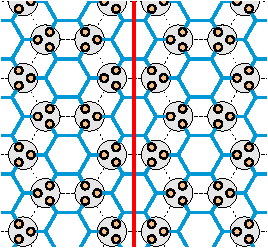
\includegraphics[width=\textwidth]{diagrams/FI_PEPS_wcut2.pdf}
			\caption{Honeycomb lattice PEPS on zig-zag cylinder with L=3, acheived by factoring W-state of plaquette bosons}
		\end{figure}
	}
	\only<4>{
	  		\begin{figure}
			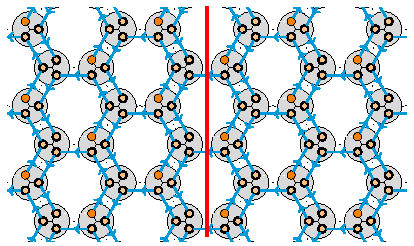
\includegraphics[width=\textwidth]{diagrams/FBI_PEPS_3.pdf}
			\caption{Honeycomb lattice PEPS on zig-zag cylinder with L=3, acheived by factoring W-state of plaquette bosons}
		\end{figure}
	}	
  \end{column}
  \begin{column}[T]{.5\textwidth}
  \vskip0.5cm
  \bi
  \item[] In cylindrical geometry:
  \item Treat state as 1D
  \item Use MPS techniques
  \item On-site translational symmetry parallel to cut
  \item Physical site dimension $4^{2L}$
  \only<3->{
  \item MPS bond dimension = Rank of $\rho_{r}$ =  $2^L$
  \item Entanglement spectrum $\{\epsilon_i\}$ defined from eigenvalues $\{\rho_i\}$ of $\rho_{r}$ via $\epsilon_i = e^{-\rho_i}$
  \item Charge and Translation represented linearly on edge
  }
  \ei
  \end{column}
\end{columns}
\end{frame}